
\section{Questions de recherche}

Un éditeur de textes tel que \emph{Microsoft Word}~\cite{word} ou
\emph{Emacs}~\cite{emacs} permet à un utilisateur de créer et d'éditer un
document. Un éditeur de texte collaboratif temps réel~\cite{ellis1991groupware}
étend la rédaction d'un document à un groupe d'utilisateurs. Chacun possède son
éditeur, voit les modifications effectuées par ses collaborateurs sur le
document, effectue ses propres changements en insérant ou en supprimant du
contenu. La mise en place de ces fonctionnalités temps réel  requière
\begin{inparaenum}[(i)]
\item un moyen de communication fiable entre les éditeurs fonctionnant sur des
  machines potentiellement distantes;
\item un moyen de représenter les documents en mémoire de telle sorte que tous
  les éditeurs affichent un même document lorsqu'ils ont reçu les mêmes
  modifications~\cite{burckhardt2014replicated, shapiro2011conflict}.
\end{inparaenum}

\begin{figure}
  \begin{center}
    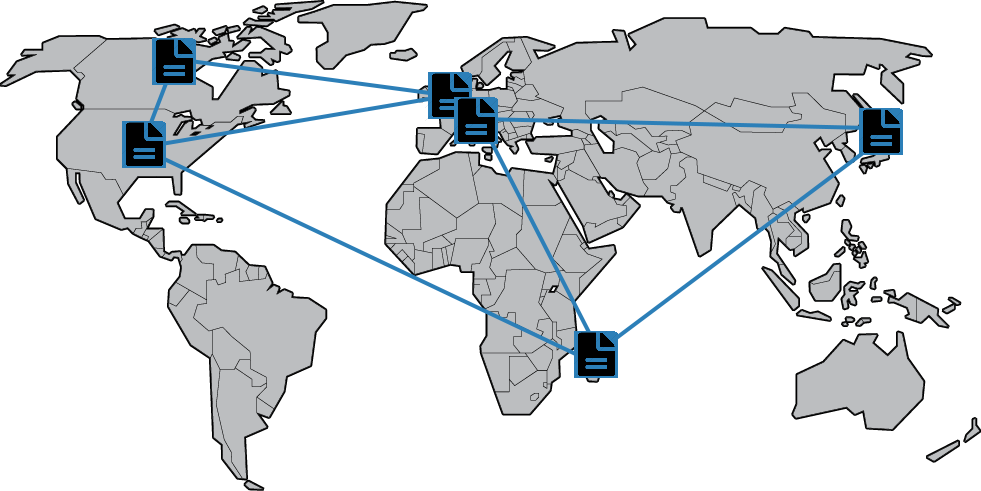
\includegraphics[width=0.85\textwidth]{img/world.png}
    \caption[Édition collaborative décentralisée]{\label{intro:img:world}Édition
      collaborative décentralisée répartie à travers le monde.}
  \end{center}
\end{figure}

La figure~\ref{intro:img:world} présente une session d'édition comprenant 6
auteurs répartis à travers le monde. Afin d'augmenter la disponibilité du
document et de diminuer le temps de réponse lors d'une modification, les
éditeurs collaboratifs actuels suivent le principe de la réplication
optimiste~\cite{saito2005optimistic}. Chaque éditeur collaboratif possède une
copie locale d'un document -- pouvant être représenté simplement par une
séquence\footnote{ou liste, ou tableau, ou série.} de caractères autorisant les
deux opérations suivantes :
\begin{inparaenum}[(a)]
\item l'insertion d'un caractère à une position dans la séquence et
\item la suppression d'un caractère à une position dans la séquence.
\end{inparaenum}
Lorsque l'utilisateur effectue une opération
\begin{inparaenum}[(i)]
\item elle est directement répercutée sur sa copie avant
\item d'être envoyée au reste des éditeurs où
\item elle est intégrée.
\end{inparaenum}


\begin{figure}
  
\begin{tikzpicture}[scale=1.2]

  \newcommand\X{30pt};
  \newcommand\Y{30pt};
  
  \draw[->](0pt,   0pt)--(10*\X,   0pt);
  \draw[->](0pt, -1*\Y)--(10*\X, -1*\Y);
  \draw[->](0pt, -2*\Y)--(10*\X, -2*\Y);
  
  \draw[fill=black](0pt, 0pt) node[anchor=east]{réplique 1 }circle(2pt);
  \draw[fill=black](0pt, -1*\Y) node[anchor=east]{réplique 2 }circle(2pt);
  \draw[fill=black](0pt, -2*\Y) node[anchor=east]{réplique 3 }circle(2pt);

  \draw(\X,2pt)--node[anchor=south]{[WERTY]}( \X,   -2pt);
  \draw(\X,2 -1*\Y)--node[anchor=south]{[WERTY]}(\X,-2 -1*\Y);
  \draw(\X,2 -2*\Y)--node[anchor=south]{[WERTY]}(\X,-2 -2*\Y);
  \small
  \draw(3* \X,2pt)--node[anchor=north]{\textsc{insert}(\DARKBLUE{Q, 0})}(3 * \X,   -2pt);
  \draw(3* \X,2 -2*\Y)--node[anchor=north]{\textsc{delete}(\DARKBLUE{\textbf{0}})}(3 * \X,-2 -2*\Y);
  \normalsize

  \draw(3* \X,2pt)--node[anchor=south]{[QWERTY]}(3 * \X,   -2pt);
%  \draw(2* \X,2 -1*\Y)--node[anchor=south]{[ ]}(2* \X,-2 -1*\Y)
  \draw(3* \X,2 -2*\Y)--node[anchor=south]{[ERTY]}( 3 * \X,-2 -2*\Y);

  \draw[->, dashed] (5*\X, 0pt) -- (15+7*\X, -1*\Y);
  \draw[->, dashed] (5*\X, 0pt) -- (7*\X, -2*\Y);

  \small
  \draw[->, dashed] (5*\X, -2*\Y) -- (7*\X,  0*\Y)
  node[anchor=south]{\textsc{delete}(\DARKBLUE{\textbf{0}})};
  \normalsize
  \draw[->, dashed] (5*\X, -2*\Y) -- (7*\X, -1*\Y);

  \draw(9*\X, 2 -0*\Y)--node[anchor=south]{[WERTY]}(9*\X,-2 -0*\Y);
  \draw(9*\X, 2 -1*\Y)--node[anchor=south]{[QERTY]}(9*\X,-2 -1*\Y);
  \draw(9*\X, 2 -2*\Y)--node[anchor=south]{[QERTY]}(9*\X,-2 -2*\Y);


%%  \draw(9*\X, 2 -0*\Y)--node[anchor=south]{[QWERTY]}(9*\X,-2 -0*\Y);
%%  \draw(9*\X, 2 -1*\Y)--node[anchor=south]{[QWERTY]}(9*\X,-2 -1*\Y);
%%  \draw(9*\X, 2 -2*\Y)--node[anchor=south]{[QWERTY]}(9*\X,-2 -2*\Y);


%%  \draw[fill=white, very thick]
%%  (0*\X, 0*\Y) node{$p_1$} +(-5pt,-5pt) rectangle +(5pt,5pt);
%%  \draw[->](-5+\X, 5+2*\Y)to[out=120,in=30](0pt,5+2*\Y); %% 6 -> 7
\end{tikzpicture}
  \caption{\label{intro:fig:ripconvergence} Répliques divergentes d'un
    document.}
\end{figure}

L'utilisation des structures de données \og classiques \fg n'est pas directement
possible du fait de la latence entre les collaborateurs. Par exemple, la
figure~\ref{intro:fig:ripconvergence} présente un exemple où un auteur insère un
caractère sur la réplique 1 en début de document pendant qu'un autre supprime un
caractère sur la réplique 3 au même endroit. Le premier auteur risque, à tort,
de voir supprimé le caractère qu'il vient d'insérer. L'état final de la réplique
2 dépend de l'ordre de réception et d'intégration des opérations. Ici, la
suppression arrivant avant l'insertion, la séquence devient \texttt{QERTY}.
Afin d'éviter de telles divergences dans l'état des répliques, de nouvelles
structures et de nouveaux algorithmes doivent être employés.

Une première famille d'approches consiste à transformer les arguments de
l'opération afin qu'elle considère les opérations intégrées
concurremment~\cite{sun1998operational}. Dans l'exemple précédent, lors de
l'intégration de la suppression par le premier éditeur, celui-ci doit réaliser
qu'un caractère a été ajouté en tête concurremment. Il doit donc modifier les
arguments de l'opération reçue afin que le caractère \texttt{W} soit supprimé,
et non plus le caractère \texttt{Q}. Toutes les répliques convergent alors vers
la séquence \texttt{QERTY}.  Détecter ces cas concurrents nécessite de
communiquer, avec chaque opération, des données dont la croissance linéaire
empêche au groupe d'éditeurs d'atteindre de large
dimensions~\cite{charronbost1991concerning, sun2009contextbased}.

Une seconde famille d'approches consiste à utiliser des structures de données
dont les opérations sont commutatives~\cite{shapiro2011conflict} et ne souffrent
donc pas de la concurrence. Pour que les opérations commutent, ces approches
associent à chaque caractère un identifiant unique et immuable.

\paragraph{Les identifiants cachés~\cite{oster2006data}.} L'opération de
suppression de caractères se contente de cacher le caractère ciblé à
l'utilisateur. La mémoire consommée par une réplique croît de manière
monotone. Les performances d'intégration des opérations s'en trouvent
diminuées. Afin d'y remédier, un protocole de ramasse-miettes
réparti~\cite{abdullahi1998garbage} doit être exécuté régulièrement pour purger
la structure des identifiants cachés. Malheureusement, cela s'avère extrêmement
coûteux~\cite{abdullahi1998garbage}.

\paragraph{Les identifiants de taille variable~\cite{weiss2009logoot}.} Les
identifiants sont des listes dont la taille, définie à la génération, peut
croître de manière linéaire par rapport au nombre d'insertions dans la
séquence~\cite{weiss2009logoot}. Cette croissance impacte négativement les
performances du système. Afin d'y remédier, un protocole de relocalisation des
identifiants doit être exécuté régulièrement~\cite{zawirskiasynchronous}. Ces
protocoles reviennent à obtenir un consensus dans un contexte
réparti. Malheureusement, leur coût s'avère également très
élevé~\cite{mostefaoui2015signature}.

Cela pose la première question de recherche : \textbf{Afin d'éviter tout
  protocole additionnel de relocalisation des identifiants, comment allouer ces
  identifiants de sorte que leur taille soit directement sous-linéaire ?}

Pour répondre à cette première question de recherche, nous avons fait
l'hypothèse d'une communication fiable : chacune des modifications doit être
reçue par l'ensemble des éditeurs collaboratifs.
%%Pour converger vers des documents identiques, tous les changements doivent
%% parvenir à tous les éditeurs.
Une manière efficace de mettre en place cette diffusion fiable et décentralisée
consiste à suivre le principe de propagation épidémique\footnote{ou propagation
  de rumeurs.}  où
\begin{inparaenum}[(i)]
\item l'éditeur effectuant un changement choisit un sous-ensemble d'éditeurs
  possédant une réplique du document et leur envoie la modification;
\item lorsqu'un éditeur reçoit un tel message, il choisit à son tour un
  sous-ensemble d'éditeurs auxquels faire suivre le message.
\end{inparaenum}
Les changements atteignent tous les éditeurs par transitivité.
% Par conséquent, un réseau superposé doit être mis en place afin de permettre une
% communication fiable d'un éditeur à l'autre.
La figure~\ref{intro:img:world} montre que chaque éditeur est connecté à
d'autres éditeurs -- ses voisins -- possédant une réplique du document. Ici,
l'éditeur localisé aux États-Unis communique avec les éditeurs canadien,
français et malgache.
% Chaque éditeur participe activement au bon fonctionnement
%du système.
Une opération émise par ce premier peut transiter par l'éditeur localisé à
Madagascar avant de parvenir à l'éditeur japonais. 
% Les changements parviennent
%à tous les éditeurs par transitivité~\cite{birman1999bimodal}.

Notre contexte nous expose à deux contraintes :
\begin{inparaenum}[(i)]
\item l'éditeur doit fonctionner dans les navigateurs Web;
\item l'éditeur doit maintenir un voisinnage dont la taille gère aussi bien les
  petits groupes que les grands.
\end{inparaenum}
% La taille des voisinages est déterminante.
En effet, lorsqu'il augmente, le trafic généré augmente au risque de dépasser
les capacités d'émission des éditeurs; lorsqu'il diminue, les changements
risquent de ne plus parvenir à tous les éditeurs.

Afin de configurer la taille de cet ensemble idéalement~\cite{erdos1959random},
le développeur doit connaître le nombre de collaborateurs que l'éditeur
collaboratif doit supporter. Malheureusement, celui-ci varie, que ce soit
pendant la durée de la collaboration, e.g., un cours de formation en ligne
(\emph{MOOC})~\cite{breslow2013studying} voit sa population fluctuer selon
l'intérêt qu'il suscite; ou entre deux documents, e.g., un document créé pour un
événement de grande ampleur n'a pas la même audience que celle d'un rapport de
projet écrit par des étudiants.

Cela pose la seconde question de recherche : \textbf{Comment adapter
  efficacement le voisinage de chaque éditeur au nombre fluctuant de
  collaborateurs?}

%%\paragraph{QR A.} \textbf{Afin d'ajuster le trafic à la session d'édition,
%%  comment adapter efficacement le voisinage de chaque éditeur aux fluctuations
%%  des réseaux?}



%%% Local Variables:
%%% mode: latex
%%% TeX-master: "../../paper"
%%% End:
